\documentclass{standalone}
\usepackage{mintikz}

\tikzset{oplus/.style={path picture={% 
            \draw[black]
             (path picture bounding box.south west) --
             (path picture bounding box.north east) 
             (path picture bounding box.north west) --
             (path picture bounding box.south east);
            }},
        process/.style={draw, diamond, rounded corners,
            fill=Orchid!30, scale=0.5},
        inout/.style={draw, rectangle, rounded corners,
            fill=cornflowerblue!20},
        inter/.style={draw, ellipse, fill=orange!40,
            scale=0.5},
        add/.style={draw, circle, oplus},
} 

\begin{document}
\begin{tikzpicture}[node distance=1cm, on grid, >=stealth']
    % Do inouts
    \node[inout]
        (data) {Donn\'ees};
    \node[inout, right=of data, xshift=1cm]
        (biascor) {BiasCor};
    \node[inout, below=of data, xshift=1cm,
         anchor=north, fill=white,
         minimum width=6cm, minimum height=5cm]
        (boxproc) {};
    \node[inout, minimum width=6cm, anchor=north, fill=Orchid!20]
        (salt2mu) at (boxproc.north) {\texttt{SALT2}$\mu$};
    \node[inner sep=0] (chainleft) at (data|-salt2mu.south) {};
    \node[inner sep=0] (chainleftop) at (data|-salt2mu.north) {};
    \node[inner sep=0] (chainright) at (biascor|-salt2mu.south) {};
    \node[inner sep=0] (chainrightop) at (biascor|-salt2mu.north) {};
    \node[inter, below=of chainleft, yshift=0.5cm]
        %(initsalt) {\texttt{SALT2}$\mu$};
    %\node[inter, below=of initsalt]
        (ab) {$\alpha$, $\beta$};
    \node[inner sep=0] (ableft) at ([shift={(-0.5cm,0)}]ab.west) {};
    \node[process, below=of chainright, yshift=0.5cm]
        (bbc5D) {\texttt{BBC5D}};
    \node[right=of bbc5D, xshift=2.5cm]
        (mcube) {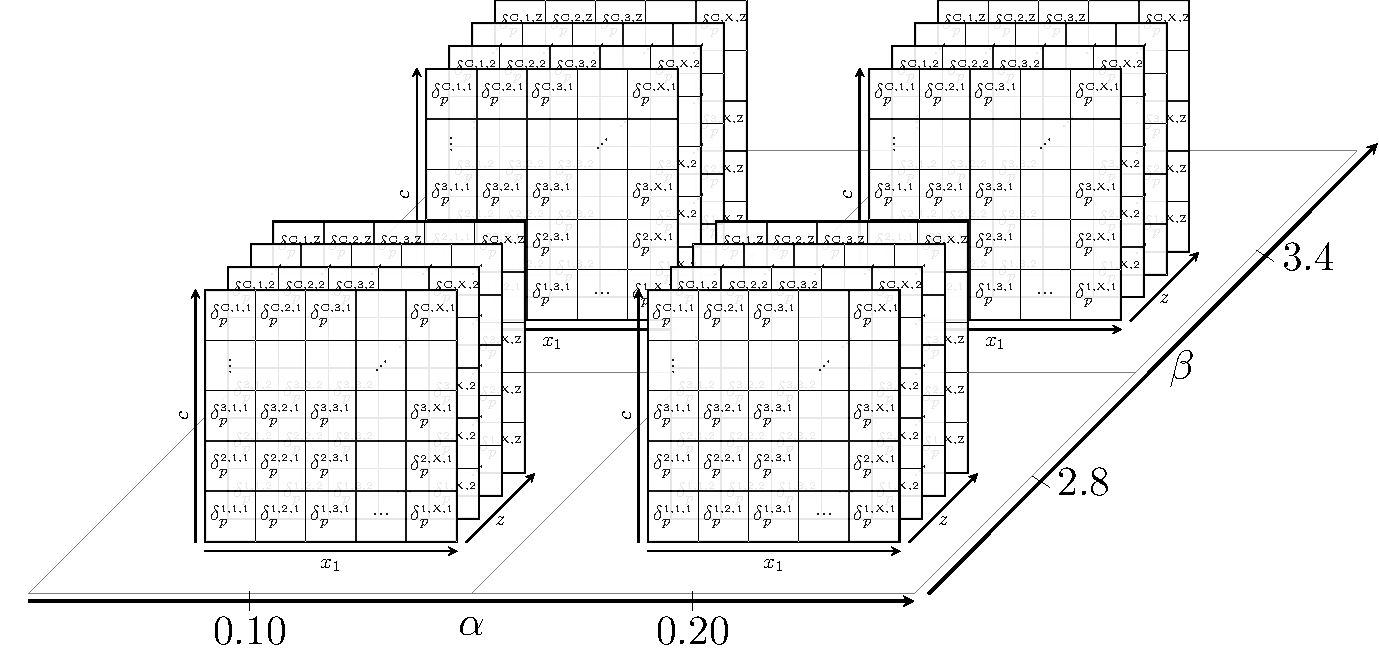
\includegraphics[width=2cm]{matrices_cube.pdf}};
    \node[inter, below=of bbc5D]
        (dbias) {$\delta\mu_{\rm biais} \equiv
                (\delta_{m_B}+\alpha\delta_{x_1}-\beta\delta_c)$};
    \node[circle, draw, fill=white, below=of salt2mu.south, yshift=-2cm]
        (chi2) {$\chi^2$};
%     \node[process, below=of biascor]
%         (bbc1D) {BBC1D};
%     \node[add, scale=2]
%         (add) at (data |- dbias) {};
%     \node[inter, below=of add]
%         (mb) {$m_B^* = m_B - \delta m_B$};
%     \node[process, below=of mb]
%         (salt2mu) {\texttt{SALT2}$\mu$};
%     \node[inter, below left=of salt2mu]
%         (ab) {$\alpha$, $\beta$};
%     \node[inout, below right=of salt2mu]
%         (res) {$z$, $\Delta\mu$};
%     \node[process, below=of res]
%         (wfit) {\texttt{wfit}};
%     \node[inout, below=of wfit]
%         (cosmo) {$w$, $\Omega_M$\ldots};
    % Plot lines
    \draw[->] (biascor) -- (chainrightop);
    \draw[->] (data) -- (chainleftop);
    \draw[->] (chainright) -- (bbc5D);
    \draw[->] (ab) -- (bbc5D);
    \draw[->] (bbc5D) -- (dbias);
    \draw[->] (dbias) |- (chi2.east);
    \draw[->, dashed] (chi2) -- (chi2 -| ableft) --
            node [diamond, draw, fill=Orchid!20, scale=0.8] {Minimisation}
            (ableft) -- (ab);
    \draw[Snake, ->, gray, dashed] (bbc5D) -- (mcube);
    % \draw[->] (dbias) -- (add);
    % \draw[->] (add) -- (mb);
    % \draw[->] (mb) -- (salt2mu);
    % \draw[->] (salt2mu) -- (ab);
    % \draw[->] (salt2mu) -- (res);
    % \draw[->] (res) -- (wfit);
    % \draw[->] (wfit) -- (cosmo);
\end{tikzpicture}
\end{document}

